%% CHANGE THIS ACCORDINGLY:
\newcommand{\authorFullName}{HAN JIE}
\newcommand{\authorUCO}{A0116448A}
\newcommand{\authorFieldOfStudy}{Electrical and Computer Engineering}
%% AND NAME THE PROJECT UCO-surname-firstname-STAT-CS-YEAR (with or without dashes)

\newcommand{\courseName}{EE5907 Pattern Recognition}

\documentclass[12pt, oneside]{report}
\usepackage[margin=0.85in]{geometry}
\linespread{1}
\usepackage{xcolor}
\usepackage[colorlinks=false, linkbordercolor=white, citebordercolor=white, 
    filebordercolor=white, urlbordercolor=white]{hyperref}
    
\usepackage{graphicx}
\usepackage[utf8]{inputenc}
\usepackage[T1]{fontenc}
\usepackage[english]{babel}

\usepackage{fancyhdr}
\pagestyle{fancy}
\renewcommand{\headrulewidth}{0.4pt}
\fancyhead{}
\fancyhead[L]{\courseName\ -- Assignment 2}
\fancyhead[R]{\authorFullName}
\fancyfoot{}
\fancyfoot[C]{\thepage}

\usepackage{titlesec}
\titlespacing{\chapter}{0pt}{*4}{*2.5}

\titleformat{\chapter}{\normalfont\huge\bf}{\thechapter}{20pt}{\huge\bf}


% definition of an environment
\usepackage{listings}
\definecolor{dgray}{gray}{0.35} % colour of R comments
\definecolor{lgray}{gray}{0.95} % background colour of R-code

\lstset{ % setting appearance of R-code
language=R, % setting language R
basicstyle=\ttfamily\small, % font and size of R-code
backgroundcolor=\color{lgray}, % background colour of R-code
commentstyle=\ttfamily\small\itshape\color{dgray}, % colour of R comments
showstringspaces=false, % forbidding the highlighting of spaces
numbers=left, % numbering on the left
numberstyle=\ttfamily\small, % font and size of numbering
stepnumber=1, % numbering with step 1
firstnumber=last, % cumulative numbering of rows in consecutive uses of lstlisting environment
breaklines=T} % automatic line breaks of code at the end of a line

\begin{document}

\begin{titlepage}
    \begin{center}
        \vspace*{1cm}
        
        \Huge
          \textbf{\courseName}
        
        \vspace{0.5cm}
        \LARGE
        Assignment 2 Face Recognition
        
        \begin{figure}[htp]
            \centering
            \includegraphics[width=10cm]{nus-logo-black-horizontal.jpg}
            \label{fig:galaxy}
        \end{figure}
        
        \vspace{1.5cm}
        \large
        SEM 1 AY2019/20
        \vspace{0.5cm}
        
        Deadline: 2400 GMT+8, Nov 24, 2019
        \vspace{1.5cm}
        
        \LARGE
        \textbf{\authorFullName}
   		  \vspace{1cm}
        
        \textbf{\authorUCO}
       
        \vfill
        
        \authorFieldOfStudy
        
        \vspace{0.8cm}
          \Large
        National University of Singapore\\
        \vspace{0.5cm}
       \today
        
    \end{center}
\end{titlepage}
\addtocontents{toc}{~\hfill\textbf{Page}\par}
\section*{1. PCA for Feature Extraction, Visualization and Classification}
\noindent Text. Commentary on the approach to solving the exercise, theoretical derivation if the assignment asks for it.

Text. Paragraphs are separated by an empty line. 

\subsection*{Implementation in R}
\begin{lstlisting}
functions in  R ...
## function for calculating basic characteristics
basicchar <- function(x){
  v1 <- c(length(x), round(mean(x),2), round(sd(x),2))
  return(v1)
}
# calculating basic characteristics of women and of men
women <- basicchar(data$skull.height[data$sex == 'F'])
men <- basicchar(data$skull.height[data$sex == 'M'])
tab <- rbind(women, men)
# plotting boxplots
boxplot(data$skull.height[data$sex == 'F'], 
        data$skull.height[data$sex == 'M'],
        col = "steelblue", 
        xlab = "",
        ylab = "Skull Height (mm)",
        xaxt = "n", 
        boxwex = 0.5)
axis(1, at = 1:2, labels = c("women","men"))
# adding averages
points(tab[,2], col = "red", pch = 16)
\end{lstlisting}

You will submit your complete code in an \textsf{.R} file or an \textsf{.Rnw} file according to the instructions for the assignments. Only required functions or parts of code crucial to the exercise will be inserted here.
\bigskip
\subsection*{Results and interpretation}
\noindent Text. Results in table or graphic form. Commentaries and interpretation of the results.

 Interpretation. Text. Commentary relating to tables and figures. What can we infere about the differences in skull height between men and women from the values in the table? How can we know from the figure, whether our data come from a normal distribution?

\begin{table}[ht]
\footnotesize
\centering

\begin{tabular}{r||rrr}
 Gender & Number of individuals & Average skull height (mm) & Standard deviation \\ 
 \hline \hline
Women & 20 & 127.70 & 6.86 \\ 
Men & 40 & 135.54 & 5.20 \\ 
\end{tabular}
\caption{Basic characteristics of skull height of women and of men}
\end{table}


\begin{figure}[ht]
\centering
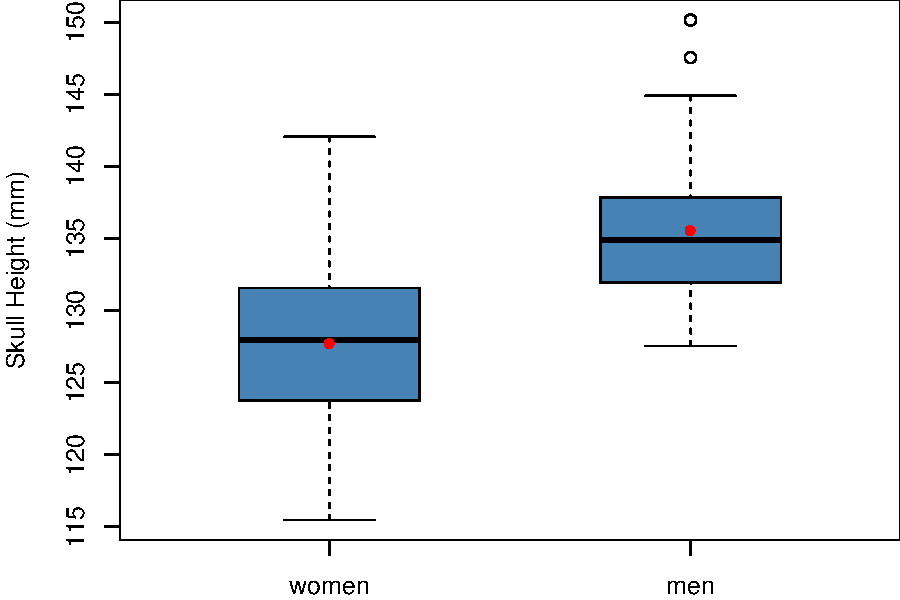
\includegraphics[angle=0,width=0.45\textwidth]{boxplot-example.pdf}
\caption{Boxplots of skull height of women and of men}
\end{figure}

\newpage

\section*{2. LDA for Feature Extraction and Classification}
\noindent Text. Commentary on the approach to solving the exercise, theoretical derivation if the assignment asks for it.

Text. Paragraphs are separated by an empty line. 

\subsection*{Implementation in R}
\begin{lstlisting}
functions in  R ...
## function for calculating basic characteristics
basicchar <- function(x){
  v1 <- c(length(x), round(mean(x),2), round(sd(x),2))
  return(v1)
}
# calculating basic characteristics of women and of men
women <- basicchar(data$skull.height[data$sex == 'F'])
men <- basicchar(data$skull.height[data$sex == 'M'])
tab <- rbind(women, men)
# plotting boxplots
boxplot(data$skull.height[data$sex == 'F'], 
        data$skull.height[data$sex == 'M'],
        col = "steelblue", 
        xlab = "",
        ylab = "Skull Height (mm)",
        xaxt = "n", 
        boxwex = 0.5)
axis(1, at = 1:2, labels = c("women","men"))
# adding averages
points(tab[,2], col = "red", pch = 16)
\end{lstlisting}

You will submit your complete code in an \textsf{.R} file or an \textsf{.Rnw} file according to the instructions for the assignments. Only required functions or parts of code crucial to the exercise will be inserted here.
\bigskip
\subsection*{Results and interpretation}
\noindent Text. Results in table or graphic form. Commentaries and interpretation of the results.

 Interpretation. Text. Commentary relating to tables and figures. What can we infere about the differences in skull height between men and women from the values in the table? How can we know from the figure, whether our data come from a normal distribution?

\begin{table}[ht]
\footnotesize
\centering

\begin{tabular}{r||rrr}
 Gender & Number of individuals & Average skull height (mm) & Standard deviation \\ 
 \hline \hline
Women & 20 & 127.70 & 6.86 \\ 
Men & 40 & 135.54 & 5.20 \\ 
\end{tabular}
\caption{Basic characteristics of skull height of women and of men}
\end{table}


\begin{figure}[ht]
\centering
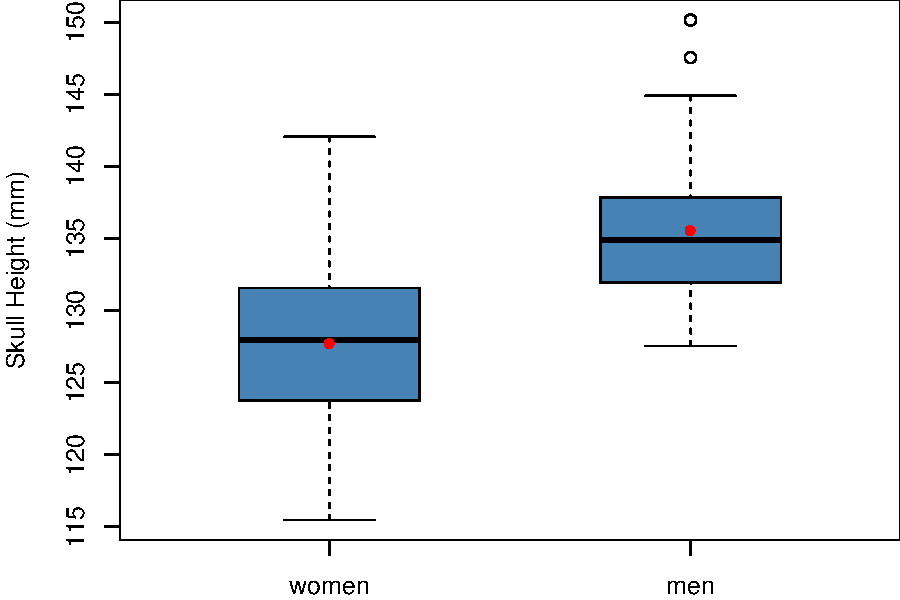
\includegraphics[angle=0,width=0.45\textwidth]{boxplot-example.pdf}
\caption{Boxplots of skull height of women and of men}
\end{figure}

\section*{3. SVM for Classification}
\noindent Text. Commentary on the approach to solving the exercise, theoretical derivation if the assignment asks for it.

Text. Paragraphs are separated by an empty line. 

\subsection*{Implementation in R}
\begin{lstlisting}
functions in  R ...
## function for calculating basic characteristics
basicchar <- function(x){
  v1 <- c(length(x), round(mean(x),2), round(sd(x),2))
  return(v1)
}
# calculating basic characteristics of women and of men
women <- basicchar(data$skull.height[data$sex == 'F'])
men <- basicchar(data$skull.height[data$sex == 'M'])
tab <- rbind(women, men)
# plotting boxplots
boxplot(data$skull.height[data$sex == 'F'], 
        data$skull.height[data$sex == 'M'],
        col = "steelblue", 
        xlab = "",
        ylab = "Skull Height (mm)",
        xaxt = "n", 
        boxwex = 0.5)
axis(1, at = 1:2, labels = c("women","men"))
# adding averages
points(tab[,2], col = "red", pch = 16)
\end{lstlisting}

You will submit your complete code in an \textsf{.R} file or an \textsf{.Rnw} file according to the instructions for the assignments. Only required functions or parts of code crucial to the exercise will be inserted here.
\bigskip
\subsection*{Results and interpretation}
\noindent Text. Results in table or graphic form. Commentaries and interpretation of the results.

 Interpretation. Text. Commentary relating to tables and figures. What can we infere about the differences in skull height between men and women from the values in the table? How can we know from the figure, whether our data come from a normal distribution?

\begin{table}[ht]
\footnotesize
\centering

\begin{tabular}{r||rrr}
 Gender & Number of individuals & Average skull height (mm) & Standard deviation \\ 
 \hline \hline
Women & 20 & 127.70 & 6.86 \\ 
Men & 40 & 135.54 & 5.20 \\ 
\end{tabular}
\caption{Basic characteristics of skull height of women and of men}
\end{table}


\begin{figure}[ht]
\centering
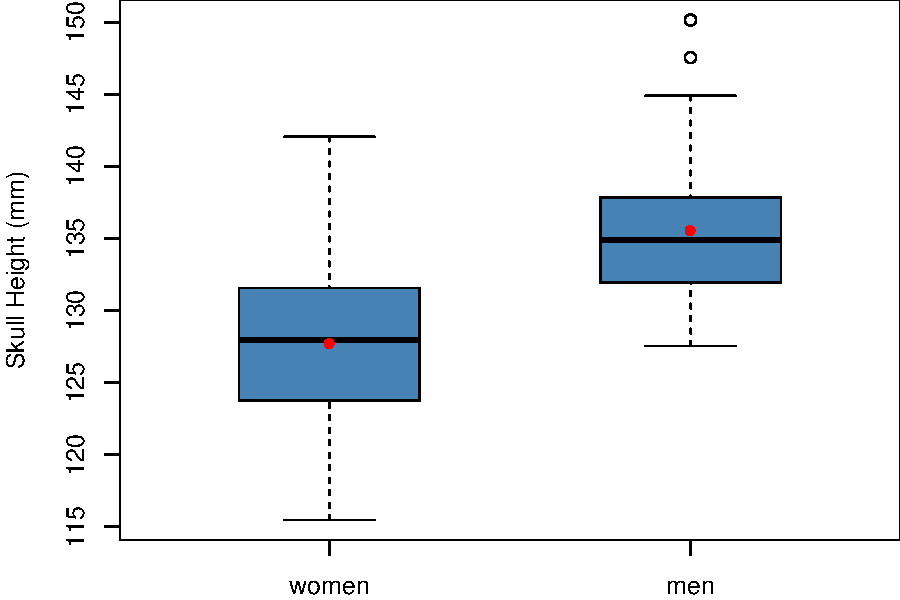
\includegraphics[angle=0,width=0.45\textwidth]{boxplot-example.pdf}
\caption{Boxplots of skull height of women and of men}
\end{figure}

\newpage

\section*{4. Neural Networks}
\noindent Text. Commentary on the approach to solving the exercise, theoretical derivation if the assignment asks for it.

Text. Paragraphs are separated by an empty line. 

\subsection*{Implementation in R}
\begin{lstlisting}
functions in  R ...
## function for calculating basic characteristics
basicchar <- function(x){
  v1 <- c(length(x), round(mean(x),2), round(sd(x),2))
  return(v1)
}
# calculating basic characteristics of women and of men
women <- basicchar(data$skull.height[data$sex == 'F'])
men <- basicchar(data$skull.height[data$sex == 'M'])
tab <- rbind(women, men)
# plotting boxplots
boxplot(data$skull.height[data$sex == 'F'], 
        data$skull.height[data$sex == 'M'],
        col = "steelblue", 
        xlab = "",
        ylab = "Skull Height (mm)",
        xaxt = "n", 
        boxwex = 0.5)
axis(1, at = 1:2, labels = c("women","men"))
# adding averages
points(tab[,2], col = "red", pch = 16)
\end{lstlisting}

You will submit your complete code in an \textsf{.R} file or an \textsf{.Rnw} file according to the instructions for the assignments. Only required functions or parts of code crucial to the exercise will be inserted here.
\bigskip
\subsection*{Results and interpretation}
\noindent Text. Results in table or graphic form. Commentaries and interpretation of the results.

 Interpretation. Text. Commentary relating to tables and figures. What can we infere about the differences in skull height between men and women from the values in the table? How can we know from the figure, whether our data come from a normal distribution?

\begin{table}[ht]
\footnotesize
\centering

\begin{tabular}{r||rrr}
 Gender & Number of individuals & Average skull height (mm) & Standard deviation \\ 
 \hline \hline
Women & 20 & 127.70 & 6.86 \\ 
Men & 40 & 135.54 & 5.20 \\ 
\end{tabular}
\caption{Basic characteristics of skull height of women and of men}
\end{table}


\begin{figure}[ht]
\centering
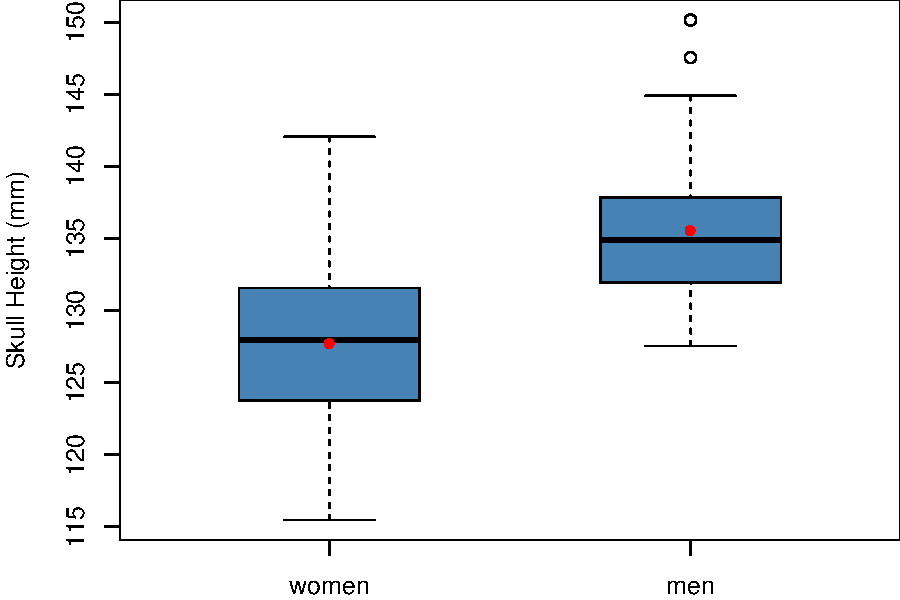
\includegraphics[angle=0,width=0.45\textwidth]{boxplot-example.pdf}
\caption{Boxplots of skull height of women and of men}
\end{figure} % inputs file with main text
\end{document}